\documentclass[conference,10pt]{IEEEtran}
\IEEEoverridecommandlockouts
\usepackage[utf8]{inputenc}
\usepackage[english]{babel}
\usepackage{amsmath,amssymb,amsfonts}
\usepackage{graphicx}
\graphicspath{./graphics/}
\usepackage{tabularx}
\usepackage{cite}
\usepackage{url}
\usepackage{enumerate}
\usepackage[dvipsnames]{xcolor}
\usepackage{wasysym}
\usepackage{gensymb}
\usepackage{tikz}
\usepackage{pgfplots}
\pgfplotsset{compat=newest}
\usepgfplotslibrary{groupplots}
\usepgfplotslibrary{dateplot}
\usepackage{macros}
\def\NewL{\\\noindent\hspace*{5mm}}
\begin{document}
\title{Detection of Constant Phase Shifts in\\Filters for Sound Field Synthesis\\
{\footnotesize Submission as abstract reviewed paper for 5th International
Conference on Spatial Audio (ICSA), Ilmenau, Germany, September 2019}}
\author{\IEEEauthorblockN{Frank Schultz, Nara Hahn, Sascha Spors}
\IEEEauthorblockA{\textit{Institute of Communications Engineering,
University of Rostock}\\
Rostock, Germany\\
\{frank.schultz, nara.hahn, sascha.spors\}@uni-rostock.de}
}
\maketitle
\thispagestyle{plain}
\pagestyle{plain}
\begin{abstract}
Filters with constant phase shift in conjunction with 3/6~dB
amplitude decay per octave frequently occur in sound field synthesis and
sound reinforcement applications.
%
These ideal filters, known as (half) differentiators, exhibit
zero group delay and 45/90 degree phase shift.
%
It is well known that certain group delay distortions in electro-acoustic
systems are audible for trained listeners and critical audio stimuli,
such as transient, impulse-like and square wave signals.
%
It is of interest if linear distortion by a constant phase shift is audible as
well.
%
For that, we conducted a series of ABX listening tests, diotically presenting non-phase
shifted references against their treatments with different phase shifts.
%
The experiments revealed that for the critical
square waves, this can be clearly detected, which generally
depends on the amount of constant phase.
%
Here, -90 degree (Hilbert transform) is comparably easier
to detect than other phase shifts.
%
For castanets, lowpass filtered pink-noise and percussion the detection rate
tends to guessing for most listeners, although trained listeners were able to
discriminate treatments in the first two cases based on changed
pitch, attack and roughness cues.
%
Our results motivate to apply constant phase shift filters
to ensure that also the most critical signals are
technically reproduced as best as possible.
%(cf. modern electronic dance music with typical crest factor of as low as 6 dB).
%
In the paper, we furthermore give analytical expressions for
discrete-time infinite impulse response of an arbitrary constant phase shifter
and for practical filter design.

\end{abstract}
\begin{IEEEkeywords}
constant phase shift, fractional Hilbert transform, audibility of phase distortion
\end{IEEEkeywords}
\section{Introduction}
\label{sec:introduction}
%
Sound reproduction systems for large audiences
are often equipped with vertical loudspeaker arrays
which shall deliver an equally pleasant acoustic experience
to the audience in terms of loudness, timbre and spatial impression.
The reproduced wavefront can be steered and shaped towards the target region
by applying delays and weights to the individual loudspeaker signals~\cite{Meyer1984a, Meyer1990}.
%
Due to the coherence of these,
the sound field typically exhibits a low-pass filter characteristic,
and thus needs to be equalized by high-pass filtering the audio input signal.
As pointed out in \cite[Ch.~3]{schultz2016diss},
the same array processing framework is used in wave field synthesis (WFS),
which has only seemingly a different goal,
namely the physical reconstruction of a desired sound field.
The loudspeaker signals for WFS are derived from
a high-frequency approximation of
the Kirchhoff-Helmholtz integral equation~\cite{spors2008revisited, zotter2013}.
%
This enables a computationally efficient implementation of WFS
which comprises of, similar to large-scale sound reproduction,
delays and weights for the individual loudspeakers
and an overall equalization filter.
%
\NewL According to the theory of WFS~\cite{spors2008revisited},
the specification of the equalization filter
depends on the geometry and shape of the loudspeaker array.
The transfer function is $i\omega$ for 3D scenarios
where 2D arrays (e.g. spherical or planar) are used.
In terms of signals and systems theory this constitutes an differentiator,
exhibiting a slope of $+6$~dB per octave
and a constant phase of $90\degree$.
For 2D scenarios using 1D arrays (e.g. circular and linear),
the filter is given as $\sqrt{i\omega}$, constituting a half-differentiator
\cite{Tseng2000,Krishna2011},
where both the slope and phase are halved to
$+3$~dB per octave and $45\degree$, respectively.
%
\NewL In practical systems, where a continuous and infinite array cannot be used,
the specification of the equalization filter has to be adjusted accordingly.
The usage of a practical array built from individual loudspeakers causes
spectral fluctuations above the so-called spatial aliasing frequency~\cite{spors2008revisited}.
Moreover, due to the finite extent of the array,
the synthesized sound field exhibits a low frequency roll off.
The high-pass filter characteristic of an ideal equalization filter
thus should be flatten out at the highest and lowest frequencies in the spectrum,
resulting in a high-pass shelving filter.
The upper limit coincides with the spatial aliasing frequency
and the lower limit is determined by the spatial extent of the array~\cite{spors2010}.
%
\NewL The digital equalization filter is typically realized either in
a finite impulse response (FIR) or
infinite impulse response (IIR) form.
FIR type equalization filters are often designed as linear phase,
while omitting the above mentioned constant phase ($90\degree$ or $45\degree$)
\cite{wierstorf2014diss, winter2019diss}.
This results in synthesized sound fields exhibiting
a negative phase shift ($-90\degree$ or $-45\degree$)
compared to the desired reference sound field
(apart from the group delay of the FIR filter).
There are also a number of IIR type equalization filters
where the constant phase spectrum is explicitly taken into account
\cite{salvador2010}
or comes as a byproduct of the minimum phase characteristics of the desired
magnitude spectrum \cite{schultz2013daga, schultz2016diss}.
The improved physical accuracy in the synthesized sound field
is well demonstrated in \cite[Fig.~9-11]{schultz2013daga}.
%
\NewL The audibility of constant phase shifts can be regarded as special issue
of the audibility of phase distortion and group delay distortion, cf.
\cite{Hansen1974_1, Hansen1974_2,Blauert1978,Suzuki1980,Lipshitz1982, Moeller2007},
often evaluated with allpass filters.
%
From these works it is known, that audibility is strongly dependent of the
signal's waveform and spectrum and the amount of the group delay in the
critical bands.
%
Generally, sensitivity for phase/group delay distortions decreases with increasing
frequency.
%
For low frequency content a different pitch and for high frequency content
ringing and different lateralization is reported for group delay distortions.
%
The polarity of highly transient signals plays a role for the audibility.
%
It was often shown, that training on phase/group delay distorted audio content
increases the sensitivity to detect them.
%
\NewL To the authors' knowledge to date,
the perceptual impact of the constant phase shift
has not been studied yet.
It is of great interest whether the existence or absence of such a phase shift
is audible, and in the special context of sound field synthesis, if this
affects the authenticity of the synthesized sound fields.
%
The paper discusses the signal processing fundamentals of discrete-time constant
phase shift in Sec.~II.
%
In Sec.~III a listening test is presented for selected audio
content and phase shifts to initially evaluate the audibility of constant phase
shifts.
%
Sec.~IV concludes the paper.

\section{Constant Phase Shifter}
\label{sec:constant-phase-shifter}
%
A constant phase shifter, also known as fractional Hilbert transformer~\cite{lohmann1996},
refers to a filter that applies a (frequency independent) constant shift $\varphi$
to the spectrum of an input signal.
This section introduces the time and frequency representations
of discrete-time constant phase shifters for aperiodic and periodic signals.
Practical implementations for the respective cases are also discussed.
Since the primary interest of the present study is the audibility of a phase shift,
the main consideration is the accuracy of the constant phase shifter
in terms of its magnitude and phase response.
Computational cost and algorithm optimization are less of a concern.

\subsection[Aperiodic Signals]{Aperiodic Signals}
\label{sec:aperiodic-signals}
%
The transfer function of a constant phase shifter
in the discrete time Fourier transform (DTFT) domain reads
\begin{align}
H(e^{i\Omega}) &=
\begin{cases}
e^{+i\varphi}, & 0 < \Omega < \pi\\
e^{-i\varphi}, & -\pi < \Omega < 0\\
\cos\varphi, & \Omega = 0, \pi
\end{cases}
\label{eq:def-dtft}
\end{align}
where $\Omega = \frac{2\pi f}{\fs}$ denotes the normalized angular frequency
for the sampling rate $\fs$.
By exploiting Euler's formula, \eqref{eq:def-dtft} can be decomposed into
\begin{align}
H(e^{i\Omega})
= \cos\varphi
- \sin\varphi\cdot\Hh(e^{i\Omega}),
\label{eq:decomp-dtft}
\end{align}
with
$\Hh(e^{i\Omega})\coloneqq-i\cdot\sgn{\Omega}$ denoting
the transfer function of the Hilbert transformer~\cite{hahn1996hilbert}.
Notice that the Hilbert transformer can be regarded
as a constant phase shifter of $\varphi=-\tfrac{\pi}{2}$.
Since $\Hh(e^{i\Omega})$ is free of DC bias~\cite[Sec.~4.2]{hahn1996hilbert},
the magnitude response of a constant phase shifter
is unity at all frequencies but $\Omega=0, \pi$,
as given in \eqref{eq:def-dtft}.
%
\begin{figure*}[t]
\centering
\includegraphics[width=\linewidth]{graphics/discrete-irs-phi-45.pdf}
\caption{Left: Impulse response of a constant phase shifter ($\varphi=-45\degree$)
described in \eqref{eq:discrete-ir}.
Center \& Right: Impulse responses of periodic constant phase shifter ($\varphi=-45\degree$)
for even and odd period $M$, described in \eqref{eq:hperi-even} and \eqref{eq:hperi-odd}, respectively.
The coefficients $h[0] = \hperi[0] = \cos\varphi$ are indicated by \stem{colzero}.
The coefficients for $n\neq 0$ indicated by \stem{colnonzero} show
the Hilbert transform part of the impulse response.}
\label{fig:discrete-ir}
\end{figure*}
%
\begin{figure*}[]
\centering
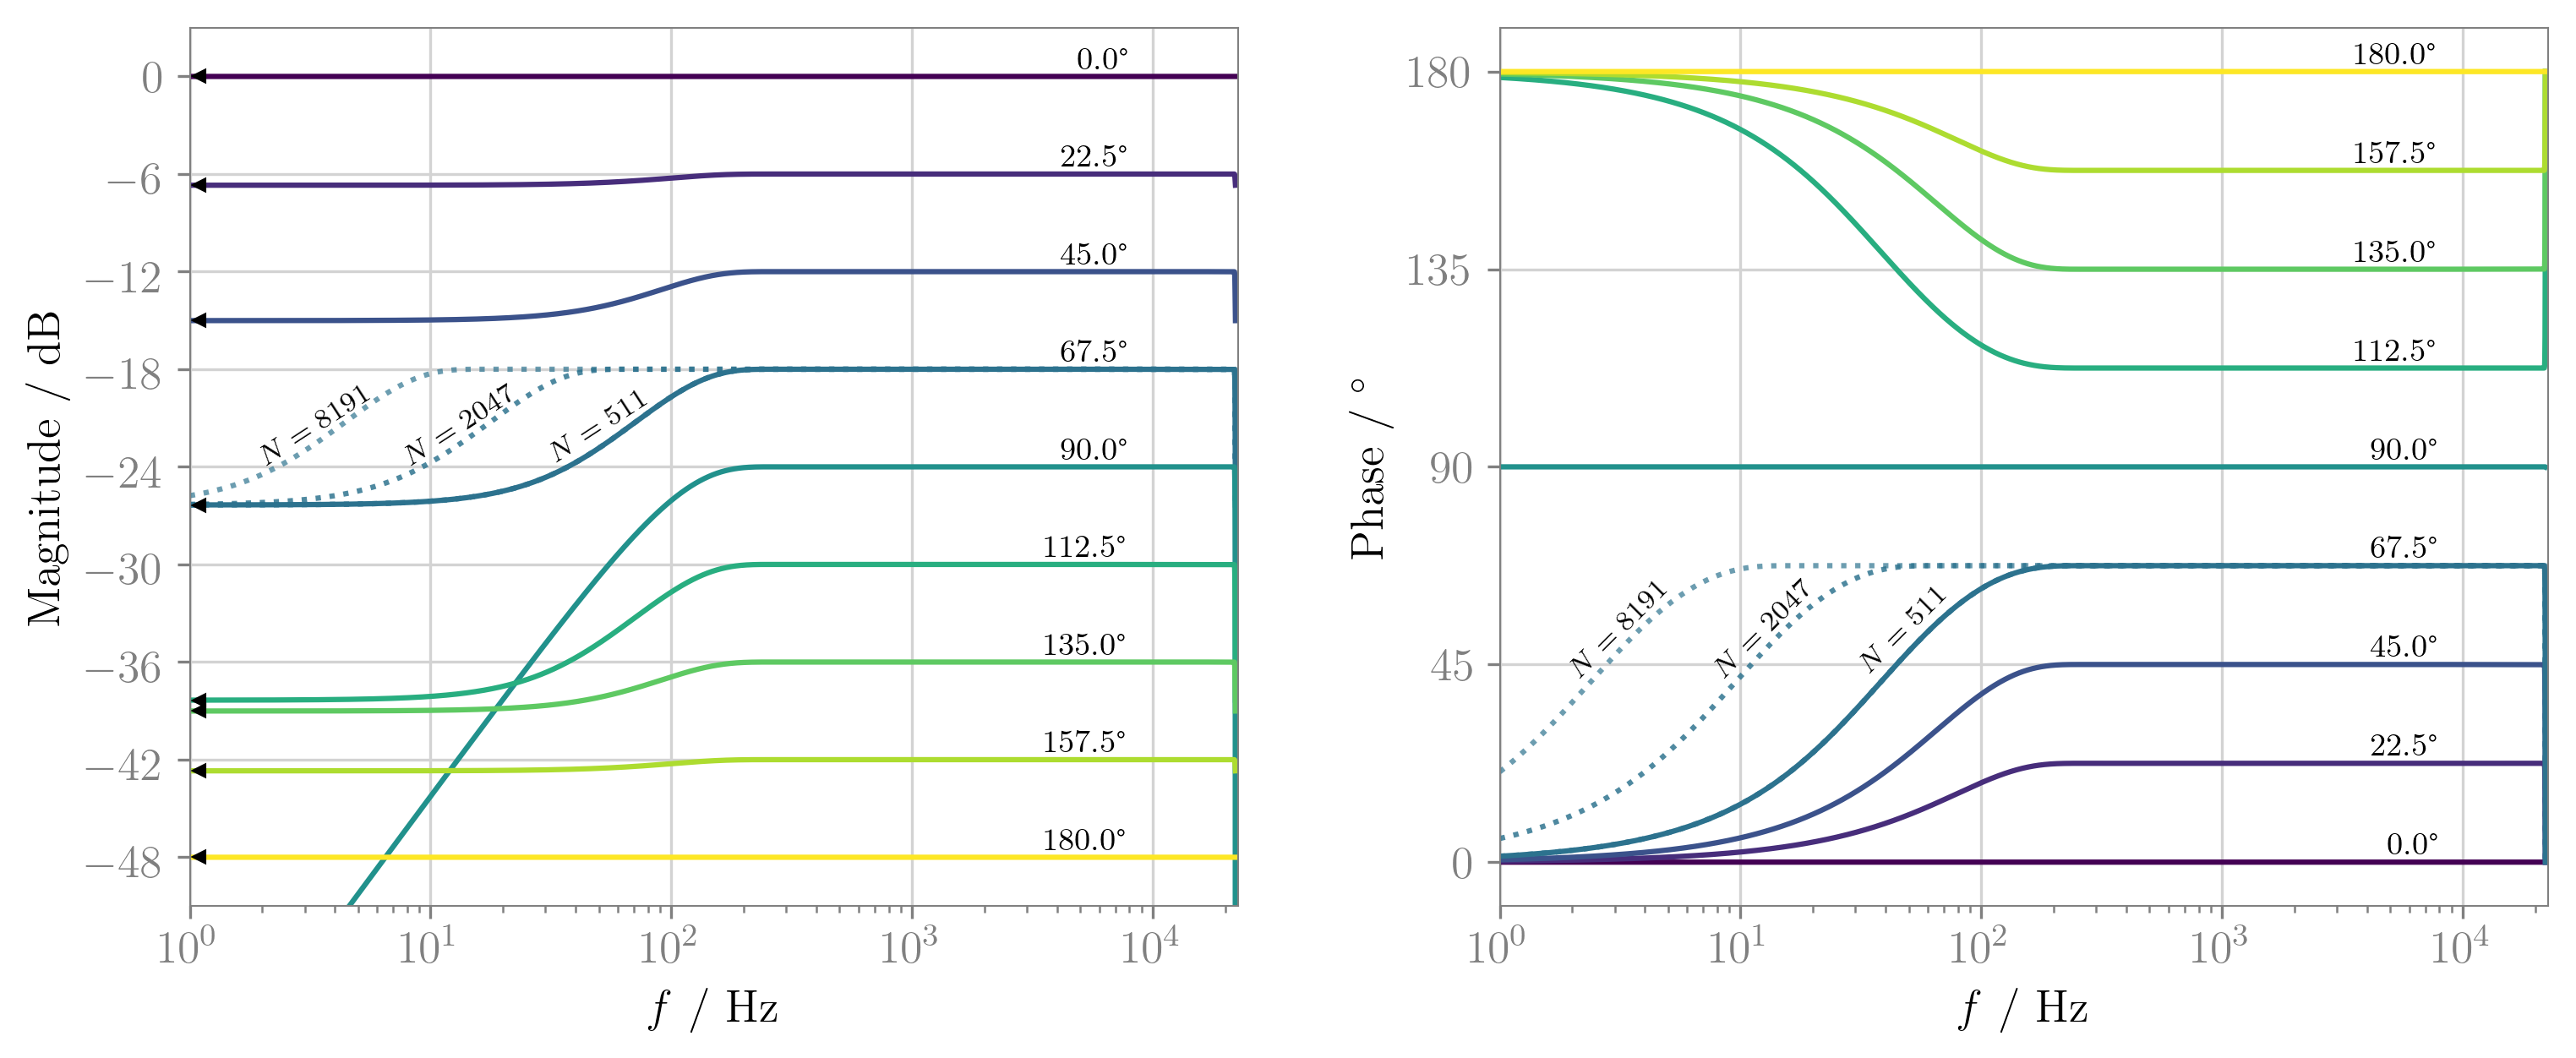
\includegraphics[width=0.85\linewidth]{graphics/spectra_filterorder510.pdf}
\caption{Frequency responses of constant phase shifters
(left: magnitude, right: phase, $\fs=44.1$~kHz).
The FIR filter coefficients are obtained by using the windowing method
(filter length of $N=511$ for all angles and $N=511, 2047, 8191$ for $\varphi=67.5\degree$).
The magnitude responses are depicted with $6$~dB offsets.
The triangles $\LHD$ indicate the DC gain $\cos\varphi$.
The phase responses are obtained by compensating the group delay
$\tau = \frac{N-1}{2}\frac{1}{\fs}$, i.e. multiplying the complex exponential
$e^{i2\pi f\tau}$ to the spectra.}
\label{fig:spectra}
\end{figure*}
%
\NewL The discrete-time impulse response of a constant phase shifter
is obtained by computing the inverse DTFT of $H(e^{i\Omega})$,
%either \eqref{eq:def-dtft} or \eqref{eq:decomp-dtft},
\begin{align}
h[n] =
\begin{cases}
\cos\varphi, & n = 0\\
0, & \text{$n \neq 0$ and even}\\
-\frac{2}{n \pi} \sin\varphi, & \text{$n$ odd}.
\end{cases}
\label{eq:discrete-ir}
\end{align}
Analogous to \eqref{eq:decomp-dtft},
it comprises of two components,
\begin{align}
h[n] &= \cos\varphi\cdot\delta[n]
- \sin\varphi \cdot \hh[n]
\label{eq:decomp-ir}
\end{align}
where
\begin{align}
\hh[n] =
\begin{cases}
0,& \text{$n$ even}\\
\tfrac{2}{n\pi},& \text{$n$ odd}.
\end{cases}
\end{align}
denotes the discrete-time impulse response of
the Hilbert transform filter~\cite[Eq.~(11.65)]{oppenheim}.
The constant phase shift of an input signal is
thus a linear combination of the input itself and its Hilbert transform,
weighted with $\cos\varphi$ and $-\sin\varphi$, respectively.
%
\NewL In Fig.~\ref{fig:discrete-ir}(left),
the impulse response $h[n]$ for $\varphi=-\tfrac{\pi}{4}$ is depicted.
It can be seen that the impulse response is
of infinite length and not causal.
The coefficients for $n\!\neq\!0$, indicated by \stem{colnonzero},
exhibit odd symmetry with respect to $n=0$ and add up to 0.
The DC and $\frac{\fs}{2}$ gain are thus solely determined by $h[0]=\cos\varphi$,
indicated by \stem{colzero}
and consistently given in \eqref{eq:def-dtft}.
%
\NewL Filtering with the impulse response $h[n]$ is not feasible in practice
due to the infinite extent of $h[n]$.
An FIR constant phase shifter can be built by applying a finite window to $h[n]$,
known as windowing method~\cite[Sec.~7.2]{oppenheim}.
Considering the decay of the coefficients for $\abs{n}\to\infty$,
it is a natural choice to truncate the impulse response
symmetrically with respect to $n=0$, which leads to
an even-order (odd-length) FIR filter.
Since $h[n]$ vanishes for even $n\neq 0$,
the FIR length $N$ has to satisfy $N\bmod 4 = 3$
(i.e. $N = 3, 7, 11, 13, \ldots$).
Using a tapering window is advantageous
as it smooths out the ripples in the frequency domain.
Due to the non-causality of the filter, a constant group delay of $\tau = \frac{N - 1}{2}\frac{1}{\fs}$
%(about the half filter length)
is introduced additionally to the desired property given by \eqref{eq:def-dtft}.
%
\NewL Exemplary frequency responses of FIR constant phase shifters
($\varphi=0\degree,\ldots,180\degree$)
are shown in Fig.~\ref{fig:spectra}.
The FIR coefficients are obtained by applying
a Blackman window to $h[n]$ in \eqref{eq:discrete-ir}.
It can be seen that the desired magnitude and phase responses
are achieved only within a limited frequency band.
For $\varphi \neq 0\degree, 180\degree$,
the magnitude responses typically
attenuate at low and high ends
($f=0$ and $f=\tfrac{\fs}{2}$, respectively)
and converge to $\cos\varphi$.
Due to the logarithmic frequency axis,
the behavior at $f=\frac{\fs}{2}$ is not clearly visible, though.
For $\varphi\neq 90\degree$,
the phase responses are inaccurate at both ends
and gradually tend to $0\degree$ or $180\degree$.
The constant phase shifter for $\varphi=90\degree$ exhibits an ideal phase response
but the most distorted magnitude response among other phase angles.
Accurate frequency responses are observed for $\varphi=0\degree, 180\degree$
where the filters are integer delays ($\tau\!=\!\frac{N-1}{2}\frac{1}{\fs}$)
with non-inverted and inverted polarity.
As indicated by dotted lines ($\varphi=67.5\degree$) in Fig.~\ref{fig:spectra},
the spectral distortions can be suppressed
by increasing the FIR filter order,
which comes at the expense of an increased group delay.

\subsection[Periodic Signals]{Periodic Signals%
\footnote{The derivation in this subsection is adopted from
\cite[Sec.~1.9 and Sec.~4.6]{hahn1996hilbert}.}}
\label{sec:periodic-signals}
%
Consider an $M$-periodic signal $\speri[n] = \speri[n + M]$
and the generating signal $s[n]$ which coincides
with $\speri[n]$ for the period $n=0,\ldots,M\!-\!1$ and vanishes elsewhere.
Then the periodic signal can be represented as a shifted sum of $s[n]$,
\begin{align}
\speri[n] = \sum_{\mu=-\infty}^{\infty} s[n] \convn \delta[n-\mu M],
\label{eq:periodic-rep}
\end{align}
where $\convn$ denotes the linear convolution with regard to $n$.
The constant phase shift of $\speri[n]$ reads
\begin{align}
\yperi[n] = \speri[n] \convn h[n]
= s[n] \convn
\underbrace{\sum_{\mu=-\infty}^{\infty} h[n-\mu M]}_{\hperi[n]},
\label{eq:periodic-conv}
\end{align}
meaning that the generating function $s[n]$ is convolved with
an infinite sum of shifted impulse responses denoted by $\hperi[n]$.
A closed form expression for $\hperi[n]$ can be obtained by
substituting \eqref{eq:decomp-ir} for $h[n]$ and exploiting
the series expansion of the cotangent function~\cite[Eq.~(4.3.91)]{abramowitz},
reading
\begin{align}
\hperi[n]=
\begin{cases}
\cos\varphi,& n=0\\
0,& \text{$n\neq 0$ and even}\\
\frac{-2\sin\varphi}{M}\cot\left(\frac{\pi n}{M}\right),& \text{$n$ odd},
\end{cases}
\label{eq:hperi-even}
\end{align}
for even $M$, and
\begin{align}
\hperi[n]=
\begin{cases}
\cos\varphi,& n=0\\
\frac{-\sin\varphi}{M} \cot\left(\frac{\pi(n + M)}{2M}\right),& \text{$n\neq 0$ and even}\\
\frac{-\sin\varphi}{M} \cot\left(\frac{\pi n}{2M}\right),& \text{$n$ odd},
\end{cases}
\label{eq:hperi-odd}
\end{align}
for odd $M$.
Exemplary impulse responses are shown
in Fig.~\ref{fig:discrete-ir}(center, right) for $\varphi=-45\degree$.
%
\NewL A periodic repetition of a signal in the time domain
is equivalent to a sampling of the spectrum in the DTFT domain~\cite[Sec.~8.4]{oppenheim}.
The discretized DTFT spectrum then constitutes
the discrete Fourier transform (DFT) spectrum~\cite[Sec.~8.5]{oppenheim},
for which periodicity of the signal and the spectrum are inherent.
The DFT coefficients for even $M$ read
\begin{align}
H[k] &= H(e^{i\frac{2\pi}{M}k})\label{eq:H-dft}\\
&= \nonumber
\begin{cases}
e^{+i\varphi},& k = 1,\ldots,\tfrac{M}{2}-1\\
e^{-i\varphi},& k = \tfrac{M}{2} + 1,\ldots, M-1\\
\cos\varphi,& k = 0, \tfrac{M}{2}
\end{cases}
\end{align}
where $H[k]$ denotes the DFT of $\hperi[n]$.
Note that \eqref{eq:hperi-even}, \eqref{eq:hperi-odd}, and \eqref{eq:H-dft}
are analytic representations of the constant phase shifter
with no approximations involved.
An ideal constant phase shift is therefore feasible
as far as periodic discrete-time signals are concerned.
%
\NewL In practice, a constant phase shift of a periodic signal
can be computed efficiently in the DFT domain,
\begin{align}
y[n] = \frac{1}{M} \sum_{k=0}^{M-1} S[k] \: H[k] \: e^{i\frac{2\pi}{M}kn},
\label{eq:dft-conv}
\end{align}
for $n=0,\ldots,M-1$, where $S[k]$ denotes the DFT of $s[n]$.
This constitutes a circular convolution of $s[n]$ and $\hperi[n]$,
and $y[n]$ exhibits a temporal aliasing which constitutes the desired result,
as shown in \eqref{eq:periodic-conv}.
Finally, the periodic signal $\yperi[n]$ is constructed
with the generating signal $y[n]$, in the same way as \eqref{eq:periodic-rep}.

%\cleardoublepage
\section{Listening Experiment}
\label{sec:listening-experiment}
%
We aim at investigating, if audio content treated with a constant phase
shift filter can be perceptually discriminated from the original signals.
%
This section discusses the design, procedure and analysis of the
conducted listening experiment, related to this question.
%
%
%
\subsection{ABX Test Framework}
The discrimination performance was tested with the highly sensitive two alternatives,
forced choice ABX test.
%
Stimuli A and X were both randomly assigned to either the reference (original)
or the treatment (phase shift), subsequently ensuring that B contains the other
stimulus than A.
%
According to the ABX test paradigm, test subjects were asked to assign either
X=A or X=B after thorough, non-time-limited comparison of A, B and X.
%
\NewL No looped playback or instantaneous stimulus switching with crossfade or
fast fade-out/fade-in could be utilized, since treatment detection would have become
a trivial task based on the resulting artifacts (i.e. clicks for fade-out/in,
phasing for crossfade).
%
Instead, the stimuli---always (re)-started from the beginning---%
had to be manually started and stopped by the test subjects.
%
This ensures artifact free playback, although with higher interaction.
%
Moreover, the requirements led to some modifications of the utilized webMUSHRA
test framework \cite{Schoeffler2018}, which by default intends seamless switching
and looping by fading out/in.
%
%
%
\subsection{Audio Content}
The 4 monaural audio contents
\begin{itemize}
\item three square wave burst signals, each: 50 Hz, 200 ms on including
40 ms $\sin^2$-fade in and out,  300 ms off.
Fourier series synthesis of the
harmonics $1, 3,\dots, 19$, modal windowing (Kaiser, $\beta=4$) of the Fourier
coefficients. total length 1.5 s @ 120 bpm, periodicity assumed~/~DFT filtering
\item pink noise\footnote{generated by Voss-McCartney algorithm:\\\url{https://github.com/AllenDowney/ThinkDSP/blob/master/code/voss.ipynb}},
lowpass filtered
(4th order Butterworth, cut frequency 300 Hz),
length 2.35 s, non-periodicity assumed~/~FIR filtering
\item castanets\footnote{anechoic version of EBU SQAM CD track 27:\\\url{https://iaem.at/Members/frank/sounds/castanets-dry} },
length 2 s, periodicity assumed~/~DFT filtering
\item Hotel California, Eagles, Hell freezes over, 1994, Geffen,
stereo version mixdown to mono, time range 0:44.938 - 0:48.142, non-periodicity assumed~/~FIR filtering
\end{itemize}
were chosen to create the 5 treatments
\begin{enumerate}[I]
\item square wave burst with $\varphi=-90\degree$
\item square wave burst with $\varphi=-45\degree$
\item lowpass filtered pink noise with $\varphi=-90\degree$
\item castanets with $\varphi=-90\degree$
\item Hotel California with $\varphi=-90\degree$,
\end{enumerate}
%
according to the following considerations:
It is known that human hearing is sensitive to group delay variations of low
frequency square wave bursts \cite{Suzuki1980}, which is assumed to hold for
constant phase shifts as well.
%
To evaluate a potential detection of phase shifts for highly transient audio
material and to check for potential detection of pre-/postringing
due to filtering of such, castanets were included.
%
Phase alignment in noise signals is highly random.
It was assumed that human hearing is sensitive to a varied phase structure of
noise with a low frequency spectrum.
%
Furthermore, a musical record with a percussion sequence---%
commonly considered as very high fidelity production (mixing: E. Scheiner,
mastering: T. Jensen)---was included.
For that content, it was assumed that a constant phase shift might be audible
in the decay of the drumheads or/and in the transients.
%
\NewL For the treatments I, II and IV signal periodicity is assumed and thus
the ideal phase shift filter via DFT (Sec. \ref{sec:periodic-signals}) was
applied.
%
To create treatments V and III, no signal periodicity was assumed for the
whole musical piece as well as for the generated pink noise raw material of 6 minutes
duration.
%
Thus FIR filtering according to Sec.~\ref{sec:aperiodic-signals} was realized.
%
Considering the audio contents as rectangularly windowed signals of infinite
duration, the filter order of 3\,963\,530 ($\approx 90\,\text{s}$!) ensures
that linear convolution of the chosen excerpt of Hotel California is complete.
%
The resulting magnitude ripple of the Blackman windowed FIR is negligible
for the relevant reproduction bandwidth.
%
Since the pink noise length can be arbitrarily set, the same FIR filter was utilized
for consistence.
%
%
%
\subsubsection{Crest Factor Discussion}
%
\begin{figure}[t]
\centering
\includegraphics[width=0.5\textwidth]{graphics/crest-factor}
\caption{Crest factor over phase shift for the 4 audio contents used in the
listening test.}
\label{fig:crestfactor}
\end{figure}
%
An ideal constant phase shifter does not alter the
spectrum of the input signal, nor does it introduce any group delay.
One noticeable technical change concerns the waveform, quantifiable in terms of
the crest factor (CF),
\begin{align}
\CF = 20 \log_{10}\left(\frac{\abs{s}_{\text{PEAK}}}{s_{\text{RMS}}}\right)\quad \text{in dB}.
\label{eq:crestfactor}
\end{align}
During the preparation of this study,
it was speculated that an increase or decrease of the CF
might lead to detectable cues (if there are any) for a phase shift.
%
\NewL Figure~\ref{fig:crestfactor} depicts the CF of the chosen audio contents
for varying phase shifts $\varphi \in [-180\degree, 180\degree]$.
For aperiodic signals (pink noise and Hotel California),
the phase shift is applied to the entire piece
but the CF is evaluated only for the selected part
which is used in the listening experiment.
Notice that the CF is $180\degree$-periodic.
This is because a phase shift of $180\degree$ reverses the polarity of the signal
and the CF remains unchanged.
Among other stimuli, the square wave burst shows the highest variation
of approximately $7$~dB.
Note, however, that due to the silence between the bursts
and the temporal shaping by the fade-in/-out window,
the CF deviates from that of a continuous square wave
(which is theoretically $\CF\!=\!0$~dB for $\varphi\!=\!0\degree, \pm180\degree$
and $\CF\!=\!\infty$ for $\varphi\!=\!\pm 90\degree$).
The CF of castanets is about $15$ to $25$~dB higher than other stimuli
because of its fast attack/decay, very short sustain,
and relatively long silence.
%
\NewL As mentioned in Sec.~\ref{sec:introduction},
phase angles of $-90\degree$ and $-45\degree$ are particularly of our interest
due to the relation with the equalization filter in WFS.
Except for square waves, a phase shift of $-45\degree$ is barely detectable
for most of the audio materials that was tested in informal listening.
Therefore, $-90\degree$ is predominantly tested in this study
whereas $-45\degree$ is included only for square wave bursts.
In Fig.~\ref{fig:crestfactor}, the CF change of the phase shifted stimuli
relative to the original signal ($\varphi=0\degree$) is annotated
above the filled circles \cflabel.

%the technical change of the signal between original and phase-shifted version
%--- i.e. change from low to high crest factor or vice versa ---
%is largest for the chosen audio material assuming a perceptual correlation.
%
%
%
\subsubsection{Audio Signal Processing and Rendering}
%
Each reference audio content (except castanets) was loudness
calibrated to -23 LUFS \cite{ITU1770}.
The according calibration gain was also applied to the associated phase shifted
stimuli.
%
Since the loudness measure of \cite{ITU1770} is suboptimal for castanets,
perceptually motivated re-calibration to -35 LUFS was pursued in order to better
match playback level with the other audio contents.
%
Non-dithered 24~Bit, 44.1~kHz PCM wav-files were rendered for all required stimuli,
carefully monitoring that amplitude clipping---as undesired artifact blended with
the phase shift---does not occur.
%
%
%
\subsection{ABX Test Statistics Considerations}
All test subjects were to rate the 5 different treatments created from the 4
audio contents in mixed, randomized order and---except for the two lead authors---%
without preliminary training or other preconditioning with respect to the research
question.
%
\NewL For each of the 5 treatments 25 ABX trials had to be rated, resulting
in $5\cdot 25=125$ judgments per test subject aiming at evaluation of
individual detection rates in the first instance.
%
Thus, with underlying Binomial distribution model
\cite{Howell2013, faul2007}, these quantities originate from
intended one-side tail hypothesis testing of the $\Hnull(p_\text{detect}=0.5)$
using Bonferroni correction to a target
rejection level $\alpha=0.05$, a target test power $1-\beta=0.95$ and an
effect size of $g=0.4$, which was determined from
preliminary test results using square wave bursts, achieving detection
probabilities of about $p_\text{detect}=0.9$.
%
\NewL Assuming independence of all collected ratings, contingency tables of
detection frequencies can be statistically evaluated with underlying Chi-Square
($\chi^2$) distribution model as post hoc tests.
%
%
%
\subsection{Experiment Procedure}
The listening test was conducted in our loudspeaker array lab with 0.3~s mean RT60
and about $40~\text{dB(A)}_\text{Leq}$
sound pressure level (SPL) of background noise.
%
A large monitor, a keyboard and a mouse were set up on a table, where test subjects
took seat in the middle of the lab during the experiment.
%
The browser based ABX GUI of the webMUSHRA software was hosted on an Apple Mac Mini
connected to an RME Fireface UC.
%
\NewL Playback was presented diotic (i.e. same signal for both ears) using
an electrodynamic, circumaural, open headphone Sennheiser HD 800.
%
Playback level was settled such that for a mono pink noise signal with
$-23~\text{LUFS}$ loudness
(%$-8.2~\text{dB}$ sample peak,
$-7.8~\text{dB}_\text{TruePeak}$,
$-21.3~\text{dB}_\text{RMS}$, i.e.
$13.5~\text{dB}_\text{CF}$)
sound pressure levels (SPLs) of
$72.7~\text{dB(A)}_\text{Leq}$ / $87.7~\text{dB(C)}_\text{Peak}$
were measured for the left and the right channel using a G.R.A.S.
headphone-to-ear coupler and a calibrated Br\"uel \& Kjaer SPL meter according
to the IEC 60318 standard.
%
\NewL 12 test subjects (4 female, 8 male) took part in the listening experiment.
Except one light tinnitus afflicted, all others reported normal hearing.
%
Test subjects' age distribution is given as $\mu_a=29.8$, $\sigma_a=6.5$ years with the
percentiles $a_{0.05}=22.6,~a_{0.25}=25,~a_{0.5}=28,~a_{0.75}=32,~a_{0.95}=40.5$ years.
%
About half of the listening test panel consists of
music production experts and (future) professional musicians
(classical instrument students).
%
The other half recruits from research related, untrained listeners,
occasionally without prior experience in performing listening tests.
%
\NewL For familiarization of the specific ABX GUI, ratings on
full band pink noise with 1~dB level difference were performed by each
test subject prior to the actual listening test.
%
This procedure was accompanied by written operational instructions and remarks,
indicating that the differences to be detected in the actual listening test might be
very subtle and will potentially differ in character compared to that of the training
session.
%
Participants (except the two authors) were left completely uninformed
with respect to the signal manipulation method, thus expecting unbiased
strategies for the detection of differences.
%
\NewL After many pre-listening experiments, we decided against playback of all
25 trials per each treatment in one sequence.
This regularly resulted in an extremely tedious task, that should only be
considered for few well trained and extraordinary performing test subjects.
%
Since, in the first instance, we intended to find effect sizes $g$ for a rather
untrained, non-preconditioned test panel, we set up playback for a mixed
randomized sequence of all 125 trials, divided in 4 parts
(35 + 3 $\cdot$ 30) with longer intermissions.
%
Thus, the results to be presented in the next section, should be
considered for this conditioning.
%
%
%
\subsection{Results}
\subsubsection{Tests on Binomial Distribution}
%
\begin{figure}[t]
\centering
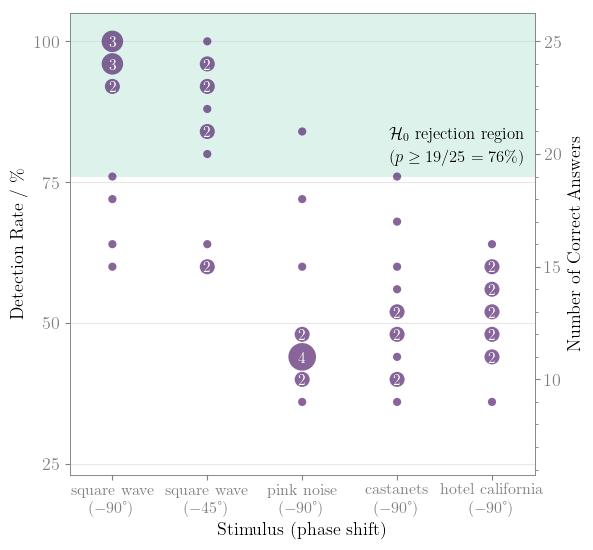
\includegraphics[width=0.5\textwidth]{graphics/scatter}
\caption{Detection rates in percent and number of
correct detections of all test panelists. Small dots without numbering indicate
a performance of a single test subject, whereas increasing dots with numbering
indicate same performance for multiple test subjects. Results within the
\colorbox{colhnull}{shaded area} indicate that guessing is unlikely with statistical significance.}
\label{fig:scatter}
\end{figure}
%
The detection rates (correct discrimination between original and phase shifted
version) of all test subjects for all treatments are shown as a scatter plot in
Fig.~\ref{fig:scatter}.
%
For the $-90\degree$ phase shifted square wave burst, except of three subjects, all
other perform with very high, statistically significant detection rates between
$76\%$ and $100\%$.
%
For the $-45\degree$ phase shifted square wave burst, except of the same  three subjects,
all other show very high, statistically significant detection rates between
$80\%$ and $100\%$.
%
\NewL The $-90\degree$ phase shifted pink noise treatment exhibits only one result
for which guessing can be excluded by statistical significance.
This was produced by one of the preconditioned, trained authors.
%
The majority of detection is slightly below guessing.
%
About the same situation, however with larger spread of the rates, can be observed
for the $-90\degree$ phase shifted castanets treatment.
The one statistically significant result was achieved by another trained,
preconditioned author.
%
All other detection rates fail to reject that guessing took place.
%
\NewL For the musical content, i.e. the percussion sequence in Hotel California,
no statistical significance can be reported.
%
Detection rates spread around the guessing rate ranging from $36\%$ to
$64\%$.

\subsubsection{Tests on Chi-Square Distribution}
The $\Hnull$~(correct and incorrect discrimination occur with equal
frequency) is tested with the $\chi^2$ test per treatment considering all judgments.
%
Bonferroni correction for total of 5 treatments to a target
$\alpha=0.05$ was considered.
%
The results indicate that this $\Hnull$ can be rejected
with very high statistical significance for the two square wave bursts,
but not for the other three treatments.
%
\NewL The $\Hnull$ (detection performance of two treatments is independent)
is tested with the $\chi^2$ test of the contingency table built from two treatments
considering all judgments.
%
Bonferroni correction for the 10 possible pairwise comparisons to a target
$\alpha=0.05$ was considered.
%
The results indicate that this $\Hnull$ can be rejected for
the pairs I vs.~III, IV, V and II vs.~III, IV, V with very high statistical
significance and odds ratios (ORs) between $4.5$ to $6.5$.
%
For the pairs I vs.~II and III vs.~IV, V and IV vs.~V we fail to reject this
$\Hnull$.
For pairwise comparison I vs.~II the $\text{OR}\approx 1.4$ indicates a very small
(however statistically not significant, $p=0.17$) tendency for a different performance.
%
For the other pairs $\text{OR}\approx 1$ indicates very comparable rating performance.
%
%
%
\subsubsection{Rating Durations}
Test subjects took between 70 and 120 minutes in total for the whole listening
experiment, including intermissions.
%
One test subject asked to split the test onto two days for improved power of
concentration.
%
\NewL The webMUSHRA software captures data for rating durations of all trials.
%
This duration is defined as the time interval from initiating the GUI for the
actual trial up to submitting the result and moving on with the next trial.
%
Thus, this duration measure includes all (potentially longer) individual
intermissions of a test subject.
%
Pure playback duration of A,~B,~X per trial,
which is considered a more useful measure, is unfortunately not available.
%
We thus report the percentiles in Table~\ref{tbl:duration} over all rating
durations $t$ in seconds without further statistic evaluation.
%
However, the table easily reveals that the median and the interquartile range---%
that should not overly affected by longer intermission intervals---%
increase following the treatment sequence I to V.
%
\begin{table}[h]
\centering
  \begin{tabular}{ l | c | c | c | c | c}
    %\hline
    treatment &  $t_{0.05} / s$ & $t_{0.25} / s$ & $t_{0.5} / s$ & $t_{0.75}/s$ & $t_{0.95}/s$\\ \hline
    I sq -90 &8.1& 12.4& 17.7& 29.2& 60.9\\ \hline
    II sq -45 &8.9& 15.3& 23.1& 39.8& 95.2\\ \hline
    III pn -90 &13.7& 19.8& 28.7& 47.4& 98.6\\ \hline
    IV cas -90 &11.5 &20.2 &30.0 &48.2 &109.7\\ \hline
    V hc -90 &12.6  &24.4 &35.9 &52.5 &104.2\\ \hline
  \end{tabular}
\caption{Percentiles of the rating duration per ABX trial.}
\label{tbl:duration}
\end{table}


\subsubsection{Qualitative Statements}
Test subjects were asked for handwritten qualitative statements (e.g. detection cues,
artifacts) during the listening experiment.
%
Since this was handled as unforced add-on not all panelists reported back.
%
However, the received statements are highly valuable and can be summarized as follows.
%
\NewL Treatments using square wave bursts were comparably very easy to detect, and
comparing both square waves, the $-90\degree$ treatment was much easier to detect than the
one with $-45\degree$.
%
Most often pitch shifts were used as cues, but also changes in envelopment and
dispersion were reported.
%
\NewL The detection of pink noise treatments was reported as very demanding.
%
Here test subjects indicated changed pitch, roughness, sharpness, subbass
structure, melody and ambience as cues.
%
For castanets test subjects reported a hard time for detection and admitted
pure guessing very often
using either the pitch or/and the characteristics of the very first transient
(change of attack, punch and crispness)
to discriminate treatment and reference.
%
No pre-/postringing artifacts were stated for the castanets.
%
%The test subject linked to the significant detection result explicitly excluded
%this as an occurring artifact on request.
%
\NewL For the percussion sequence (Hotel California) most reports agreed on pure guessing.
%
However, test subjects also reported there to use changed decay of drumheads and
changed pitch as cues as well as smeared transients.
%
\NewL One test subject reported that A,B and X were perceived with different pitches
for the square wave bursts.
%
Here, due to the forced choice design, the achieved detection rates
must fail to reject $\Hnull$, which was confirmed post-hoc.

\section{Conclusion}
\label{sec:conclusion}
This study exhibits explorative character to firstly evaluate
the audibility of constant phase shifts.
%
For signals with rather complex structure, arbitrary constant phase shifts can only
be realized with digital signal processing.
%
Based on the Hilbert transform (i.e. the special case of $-90\degree$ constant
phase shift with unit magnitude), for which the infinite impulse responses
are well known in continuous-time and discrete-time signal domain, this paper
introduces the discrete-time infinite impulse response for an arbitrary constant
phase shifter.
%
For practical implementations an FIR design is proposed with special attention
to retain unit magnitude.
%
Furthermore, for periodic signals a periodic convolution is discussed.
%
Under the periodicity assumption, hereby the ideal phase shift filter without any
approximations or limitations can be applied.
%
The periodic convolution can be computed within DFT domain with high performance,
for which the spectrum of the constant phase shifter is given.
%
\NewL The results of the conducted listening experiment can be referred to the following
deductions.
%
Untrained, unconditioned listeners that have been repeatedly confronted with
multiple low frequency square wave bursts, lowpass filtered noise,
a transient castanet rhythm and a percussion sequence in a randomized sequence,
in general show different detection performances of applied constant phase shifts.
%
\NewL The majority of listeners was able to discriminate constant phase shifts
of $-90\degree$ and $-45\degree$ for square wave bursts with comparably little
demand and very high detection rate.
%
A 100\% detection rate was achieved by musical experts.
%
These findings are according to the known results with respect to other
low frequency group delay distortion of square waves.
%
\NewL For pink noise the majority of listeners is not able to detect constant
phase shift treatments of $-90\degree$.
%
However, the results indicate that by musical background and audio expertise
higher detection rates can be achieved, that might be tested for statistical
significance by a more sensitive test design.
%
An adapted effect size of about $g=0.2$ to $0.25$ seems to be reasonable for this.
%
The same observation and conclusion holds for the $-90\degree$ constant phase shift
of the castanets signal.
%
For both signals trained listeners are able to detect the treatment with statistical
significance.
%By intense training an effect size of about $g=0.4$, i.e. our
The initial guessed effect size can be well assumed for both
stimuli.
%
\NewL All listeners were not able to detect constant phase shift of $-90\degree$
for the sequence containing percussion material with full audio bandwidth.
%
Here, highest judgment demand was reported by qualitative statements, very
often admitting pure guessing.
%
The comparably longest rating durations might reflect this fact as well.
%
This insensitivity might be due to complex spectrum and full audio bandwidth,
compared to the other used audio contents.
%
An adapted effect size of about $g=0.15$ seems to be an appropriate choice for
a more sensitive test design (e.g. addressing significant detection rates
$\frac{\geq 69\,\text{correct}}{119\,\text{total}}$ of single treatment
judgment for $\alpha=\beta=0.05$).
%
\NewL Although, here only shown in an ABX comparison scenario and not yet for
musical contents, we cannot fully exclude that
very critical, trained listeners are able to detect constant phase shifts of
well known references even in an non-comparison task as well.
%
Considering this circumstance and the current listening experiment results,
it appears advisable to apply constant phase shift filters in 2.5D and 3D sound
field synthesis applications to perfectly guarantee that
potentially audible phase shift artifacts will not occur.

\section*{Open Science}
This project is following the open science paradigm.
%
Please find all relevant code and data in the related git repository\footnote{
https://github.com/spatialaudio/audibility-constant-phase}.
%
The DOI \url{https://doi.org/10.5281/zenodo.3383286} is directly related to the repository's state
when submitting the paper.
%
The repository includes Jupyter notebooks for signal processing calculus and
statistical evaluation, stand-alone Python code to create all presented figures,
the tex source code for the paper and the related talk, the
raw data from the listening experiment, the code modifications of the used ABX
software as well as the ABX configuration files.
%
Besides the copyrighted piece of music, all other audio content used for the
listening experiment is freely available.

\renewcommand\refname{}
\section{References}
\bibliographystyle{IEEEtran}
\bibliography{bibliography}

\section*{Submitted Abstract}
The submitted abstract slightly varies from the final abstract, since not all
referred results found their way into the final version of the paper.
Therefore, we provide the submitted abstract as follows:
%
\NewL Filters with constant phase shift, often in conjunction with +-3/6 dB
amplitude decay per octave, frequently occur in sound field synthesis and
sound reinforcement applications.
%
These ideal filters are known as (half) differentiators/integrators and exhibit
zero group delay and +-45/90 degree phase shift.
%
It is well known that certain group delay distortions in electro-acoustic
systems are audible for trained listeners for critical audio stimuli, such as
transient, impulse-like and square wave signals.
%
It is of interest if linear distortion by a constant phase shift is audible
as well.
%
For that, we conducted a series of ABX listening tests, diotically presenting
non-phase shifted references against their treatments with different phase
shifts.
%
The experiments revealed that (similar to group delay) for the critical
square waves, this can be clearly detected, which generally depends on the
amount of constant phase.
%
Here, -90 degree (Hilbert transform) is comparably easier to detect than other
phase shifts. For castanets and pink-noise shaped Dirac impulse, the detection
rate tends to guessing for most listeners, although the polarity inversion
(+-180) is detectable, thereby confirming earlier studies on this topic.
%
Our results motivate to apply constant phase shift filters to ensure that also
the most critical signals are technically reproduced  as best as possible
(cf. modern electronic dance music with typical crest factor of as low as 6 dB).
%
In the paper, we furthermore give the analytical expressions for continuous
and discrete-time infinite impulse responses for unit magnitude filter with
arbitrary constant phase shift.

Submitted: Jun 23, 21:37 GMT

Last update:Jun 24, 07:06 GMT
\end{document}
